%File: formatting-instruction.tex
\documentclass[letterpaper]{article}
\usepackage{aaai}
\usepackage{times}
\usepackage{helvet}
\usepackage{courier}
\usepackage{hyperref}
\usepackage{comment}
\usepackage{graphicx}
\usepackage{natbib}
\frenchspacing
\setlength{\pdfpagewidth}{8.5in}
\setlength{\pdfpageheight}{11in}
\pdfinfo{
/Title (Mobile Indoor Localization)
/Author (Daqing Yi)}
\setcounter{secnumdepth}{0}  
 \begin{document}
% The file aaai.sty is the style file for AAAI Press 
% proceedings, working notes, and technical reports.
%
\title{Mobile Indoor Localization}
%\subtitle{CS 660 Computer Networks}

\author{Daqing Yi\\
Brigham Young University \\
\emph{dqyi11@gmail.com}
}
\maketitle

\section{Introduction}

An \emph{Indoor positioning system} locates the objects or people in an indoor environment.
The information used for localization includes radio waves, magnetic fields, acoustic signals or other sensory information from mobile devices.

Indoor localization enables indoor navigation in shopping malls, indoor location-based advertisements, friends and family member tracking and etc.

\begin{comment}
GPS
\cite{Nirjon:2014:CIL:2594368.2594378} 
WiFi
\cite{Sen:2013:AMR:2462456.2464463}
Acoustic beacon
\cite{Liu:2013:GEF:2462456.2464450}

\cite{Rai:2012:ZZC:2348543.2348580}

\cite{Wang:2012:NNW:2307636.2307655}
Graphical model
\cite{Nandakumar:2012:CLD:2348543.2348579}
\end{comment}

\section{GPS assisted localization}
\label{sec:gps_local}

GPS has been applied widely into the 
Due to low signal strength and multipath effect, usually the GPS receiver does not work well in an indoor building.
The indoor signal strength can be reduced 10 to 100 times of that in outdoor.

\cite{Nirjon:2014:CIL:2594368.2594378} proposes a hardware-software approach \emph{COIN-GPS}, which is a highly-sensitivity cloud-offloaded instant GPS.
It consists of three components,
\begin{itemize}
	\item a directional antenna,
	\item a robust acquisition algorithm and
	\item a multi-directional location estimation algorithm.
\end{itemize}

\subsection{Robust acquisition}
Because of the signal noise, the peak detection in common acquisition becomes difficult.
The use of a directional antenna helps reduce the noise.

\subsection{Multi-direction location estimation}



\section{Wifi assisted localization}

Another popular way of localization is using WiFi signal. 
Signal strength(\emph{RSSI}) is used to estimate the distance to the AP, but it is hard to discriminate between multipath reflections and the direct path.
In \cite{Nirjon:2014:CIL:2594368.2594378}, \emph{CUPID} is proposed by leveraging PHY layer information along with natural human mobility.
\begin{figure}
	\centering
	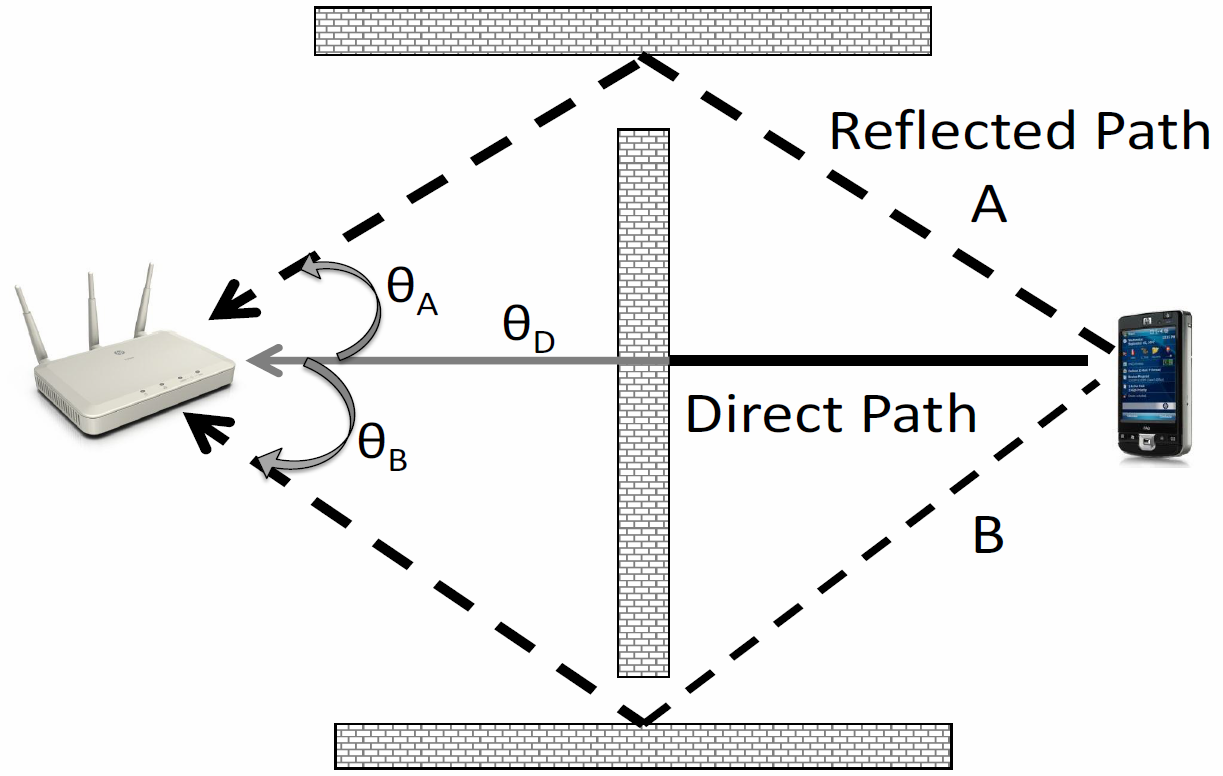
\includegraphics[width=0.7\linewidth]{fig/multipath.png}
	\caption{An example of multiple paths of wireless signal~\cite{Sen:2013:AMR:2462456.2464463}.}
	\label{fig:multipath}
\end{figure}
The localization problem becomes the estimation of the distance and the angle.
The distance estimation is obtained by \emph{EDP} (Energy of the directed path) instead of \emph{RSSI}, because it is less susceptible to mutipath reflection
\footnote{Figure \ref{fig:multipath} gives an example of multipath reflection.}.
It is extracted from \emph{CSI} (Channel state information) in the PHY layer. 
Experiments have been taken to show that this method provides a better accuracy of distance estimation than \emph{RSSI}, which the mean error is reduced from $ 10 $m to $ 4 $m.
The angle estimation is usually from \emph{AoA} (angle-of-arrival).
Usually the angle of the highest peak in MUSIC's pseudospectrum is selected as the angle of the directed path.
However, if the directed path is not blocked, the peak might correspond to a reflected path, as in Figure \ref{fig:multipath}.
The angle estimation is calculated by \emph{ANDP} (Angle of the directed path).
\begin{figure}
	\centering
	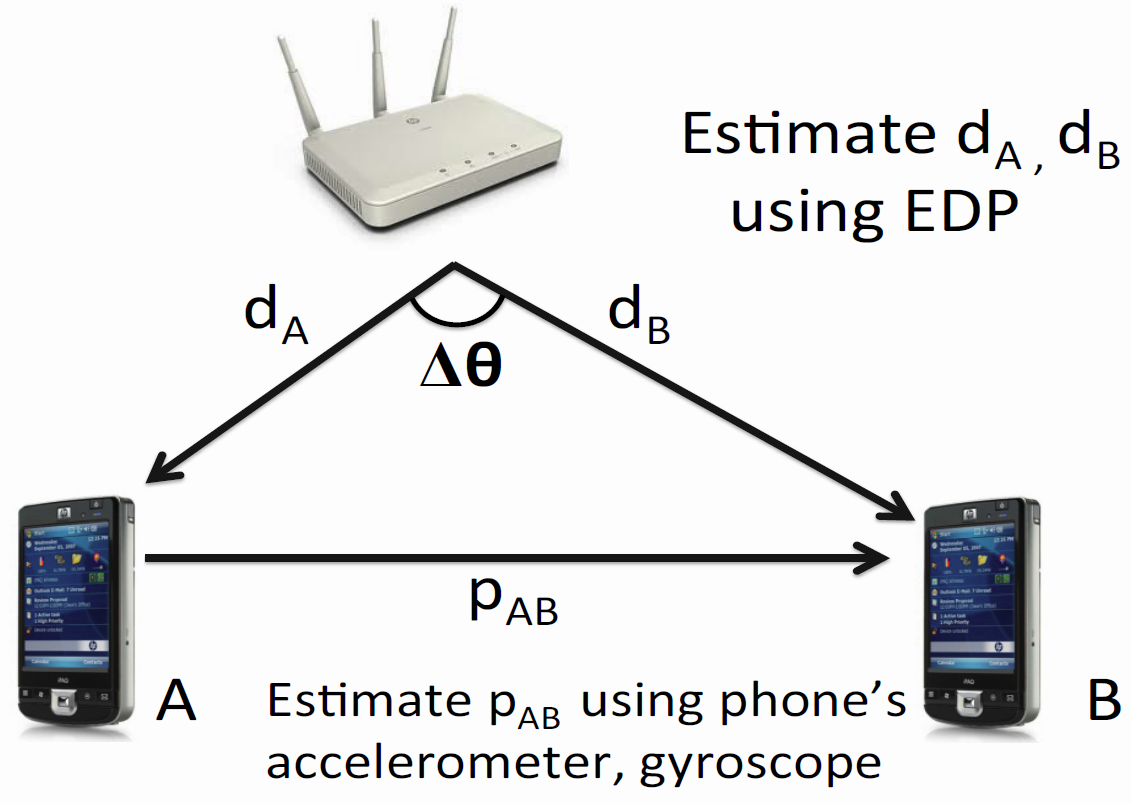
\includegraphics[width=0.7\linewidth]{fig/ANDP.png}
	\caption{Compute the change of angle using human mobility~\cite{Sen:2013:AMR:2462456.2464463}.}
	\label{fig:andp}
\end{figure}
Figure \ref{fig:andp} illustrates the calculation of
\begin{equation}
\Delta \theta = \arccos \frac{ d_{A}^{2}+d_{B}^{2}-p_{AB}^{2} }{ 2 * d_{A} * d_{B} }.
\end{equation}
The location distance $ p_{AB} $ can be obtained by the accelerometer and gyroscope of the mobile phone.

\section{Acoustic beacon assisted localization}

In \cite{Liu:2013:GEF:2462456.2464450}, an anchor network is imported for localization, which is named \emph{Guoguo}
\footnote{``Guoguo'' means Tettigonia in Chinese.}.
An anchor could transmit the spatial beacon signal to inform the unique location.
The use of acoustic communication brings
\begin{itemize}
	\item improved scalability and efficiency,
	\item and reduced hardware requirement.
\end{itemize}
\begin{figure}
	\centering
	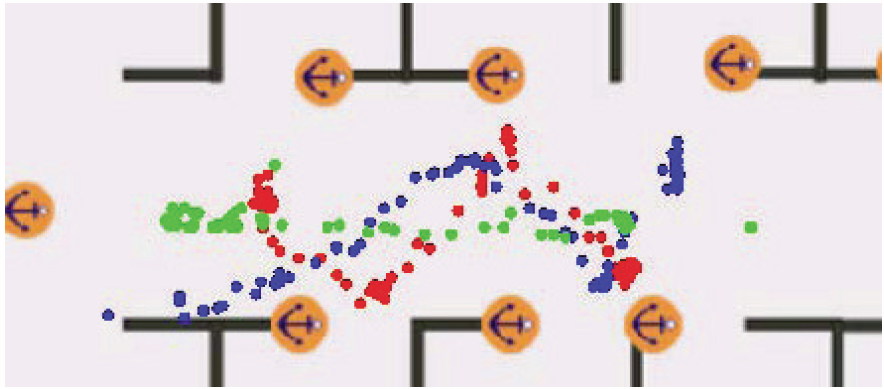
\includegraphics[width=0.9\linewidth]{fig/GUOGUO.png}
	\caption{An anchor network of Guoguo ecosystem.~\cite{Liu:2013:GEF:2462456.2464450}.}
	\label{fig:guoguo}
\end{figure}
The operation band is chosen as $ 15 kHz \sim 20 kHz $, which the human's ears are less sensitive to.
Because the beacon signal is wide-band modulated, it is unnoticeable to the humans.
All the anchor nodes are synchronized by a controller.
	
By minimizing the square errors, the position could be estimated.


\section{Hybrid information assisted localization}

\cite{Nandakumar:2012:CLD:2348543.2348579} proposes a sensory information fusion for location estimation by using Bayesian inference.
In this paper, Radio Frequency (RF) and Acoustic Ranging (AR) are used for measurement.

\emph{EchoBeep} is introduced to make AR more robust in non-line-of-sight setting.

\emph{DeafBeep} is proposed to adapt AR to localize speaker-only devices.

\section{Active learning based localization}

\cite{Rai:2012:ZZC:2348543.2348580} proposed \emph{Zee} as an active learning procedure for location estimation.
Instead of a labor intensive training set generation process, zero-effort crowdsourcing is reached.
\emph{Zee} uses WiFi and inertial sensor measurements crowdsourced from the users' smartphones to automatically infer location over time and thereby generate a WiFi training set.



\section{SLAM-based localization}

In \cite{Wang:2012:NNW:2307636.2307655}


\section{Summary}

\bibliographystyle{abbrv}
\bibliography{reference}

\end{document}
